\documentclass[conference]{IEEEtran}
\IEEEoverridecommandlockouts
% The preceding line is only needed to identify funding in the first footnote. If that is unneeded, please comment it out.
\usepackage{cite}
\usepackage{amsmath,amssymb,amsfonts}
% \usepackage{algorithmic}
\usepackage{algorithm}
\usepackage{algpseudocode}
\usepackage{graphicx}
\usepackage{textcomp}
\usepackage{xcolor}
\usepackage[numbers]{natbib}
\usepackage[normalem]{ulem}
% \documentclass[conference]{IEEEtran}
\usepackage{tabularx} % Load the package

\usepackage{cuted}
\setlength\stripsep{3pt plus 1pt minus 1pt}

% \usepackage[ruled,linesnumbered]{algorithm2e}
\usepackage{algorithm}% http://ctan.org/pkg/algorithm
\usepackage{algpseudocode}% http://ctan.org/pkg/algorithmicx

\newcommand{\heading}[1]% #1 = text
{\par\vskip 1.5ex \@plus .2ex
 \hangindent=1em
 \noindent\makebox[1em][l]{$\,\bullet$}\textbf{\large #1}%
\par\vskip 1.5ex \@plus .2ex
\@afterheading}


\def\BibTeX{{\rm B\kern-.05em{\sc i\kern-.025em b}\kern-.08em
    T\kern-.1667em\lower.7ex\hbox{E}\kern-.125emX}}
\begin{document}

\title{Reinforcement Learning for Short Range Path Planning in Indoor Environment\\
{\footnotesize \textsuperscript{}}}

\author{\IEEEauthorblockN{Prasanna Natu}
\IEEEauthorblockA{\textit{MS Robotics Engineering} \\
\textit{pvnatu@wpi.edu}\\}
%
\and
%
\IEEEauthorblockN{Shreya Bang}
\IEEEauthorblockA{\textit{MS Robotics Engineering} \\
\textit{srbang@wpi.edu}\\}
\linebreakand
\and
\IEEEauthorblockN{Shambhuraj Mane}
\IEEEauthorblockA{\textit{MS Robotics Engineering} \\
\textit{samane@wpi.edu}\\}
\and
\IEEEauthorblockN{Vaibhav Kadam}
\IEEEauthorblockA{\textit{MS Robotics Engineering} \\
\textit{vkadam@wpi.edu}}
}

\maketitle
% \begin{abstract}
  
%     % Additionally, we employ an A* Multi-Agent Path Finding (MAPF) algorithm, optimized for differential drive robot constraints, showcasing promising preliminary results
% \end{abstract}



\section{Introduction}
 Path planning of robot in an indoor environment is a crucial task of autonomous navigation, where the robot subsequently plans path from its initial state to a target state in a grid or map. Many of the path planning algorithms are not actually used on real-time robots due to its computational demands and high dimensional problems. As the advancement in Robotics, Deep Reinforcement Learning (DRL) provides a powerful tool to provide optimal path planning in deterministic indoor environments. In comparison of classical path planning algorithms, reinforcement learning (RL) based approaches have received significant attention in the recent past due to the success of the deep learning. 
 \par We provide a report for the RL based path planning for short range given a target state (pose). The robot is equipped with a 2D Lidar sensor, RL-based path planner provides optimal paths to given target pose independent of map environmennt.
 Our contribution is to plan paths using Proximal Policy Optimization (PPO) and 
 Actor Critic (A2C) implementation.





\begin{figure}[!htb]
\centering
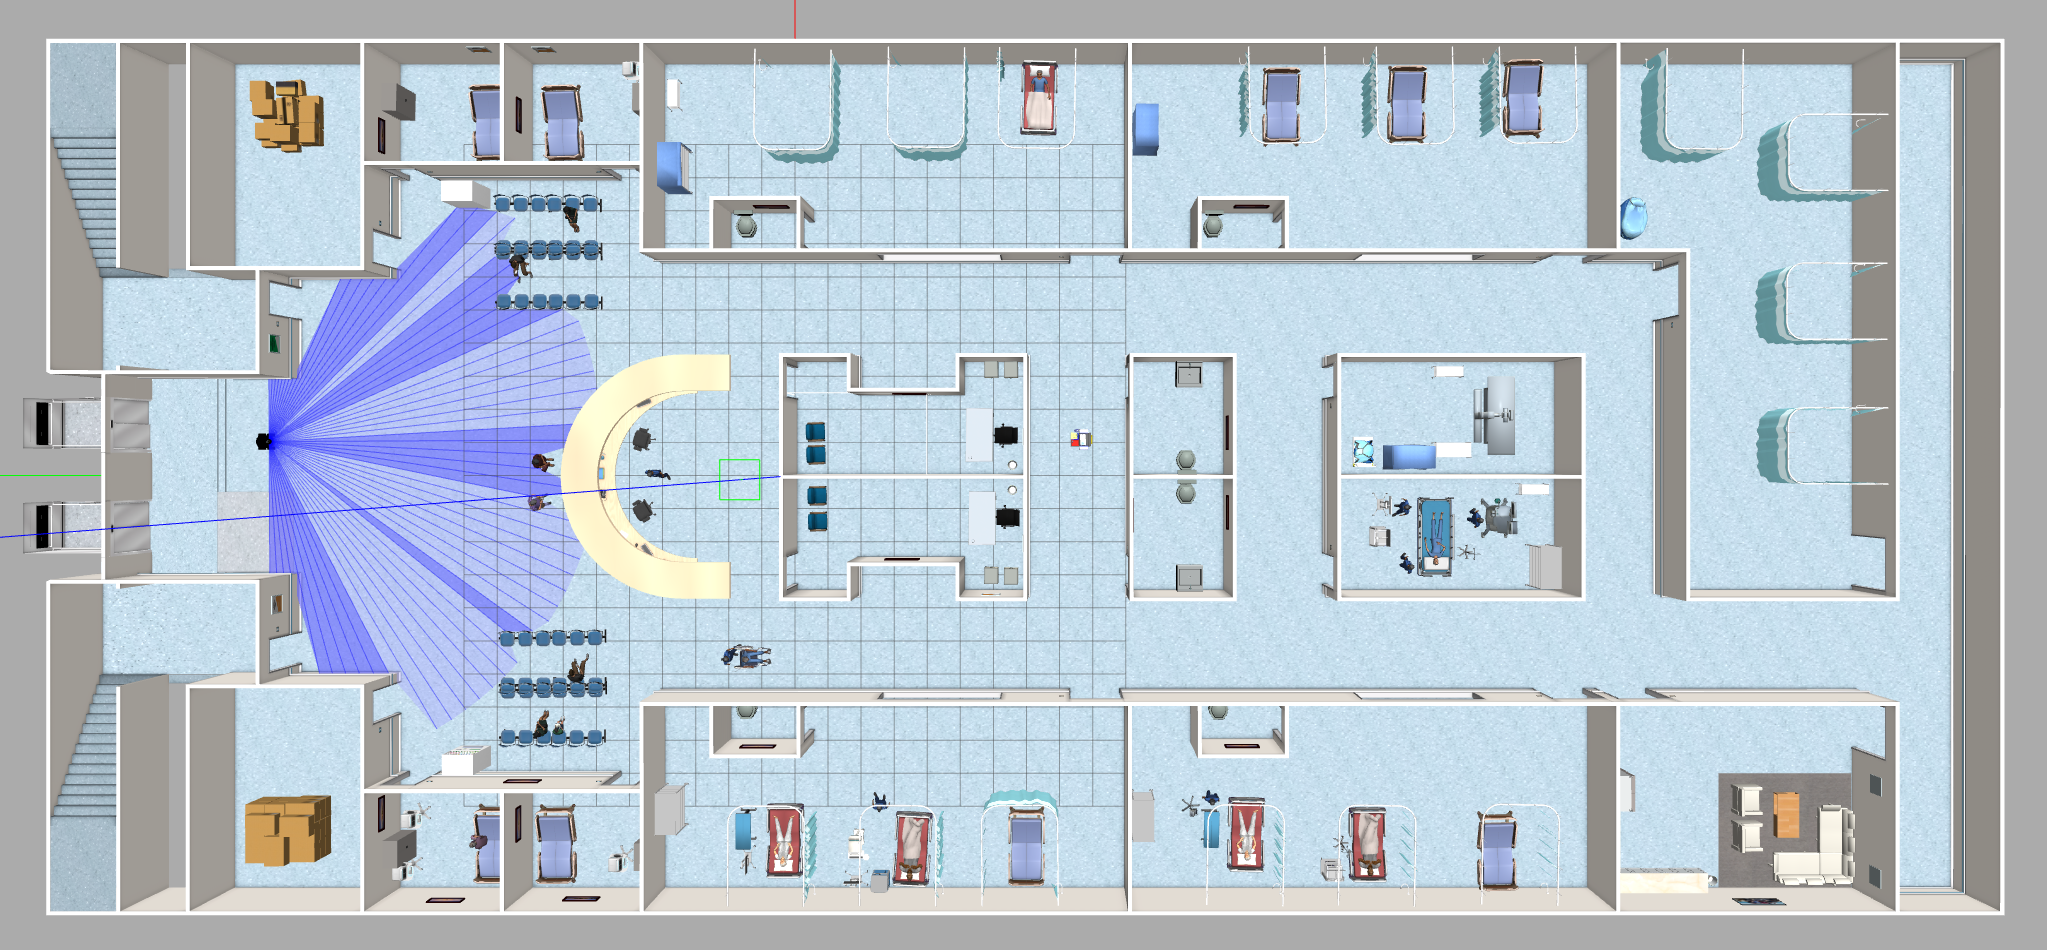
\includegraphics[width=0.8\columnwidth,keepaspectratio]{env.png}
\caption{Gazebo Hospital Environment }
\label{fig:your_label}
\end{figure}
\begin{figure}[!htb]
\centering
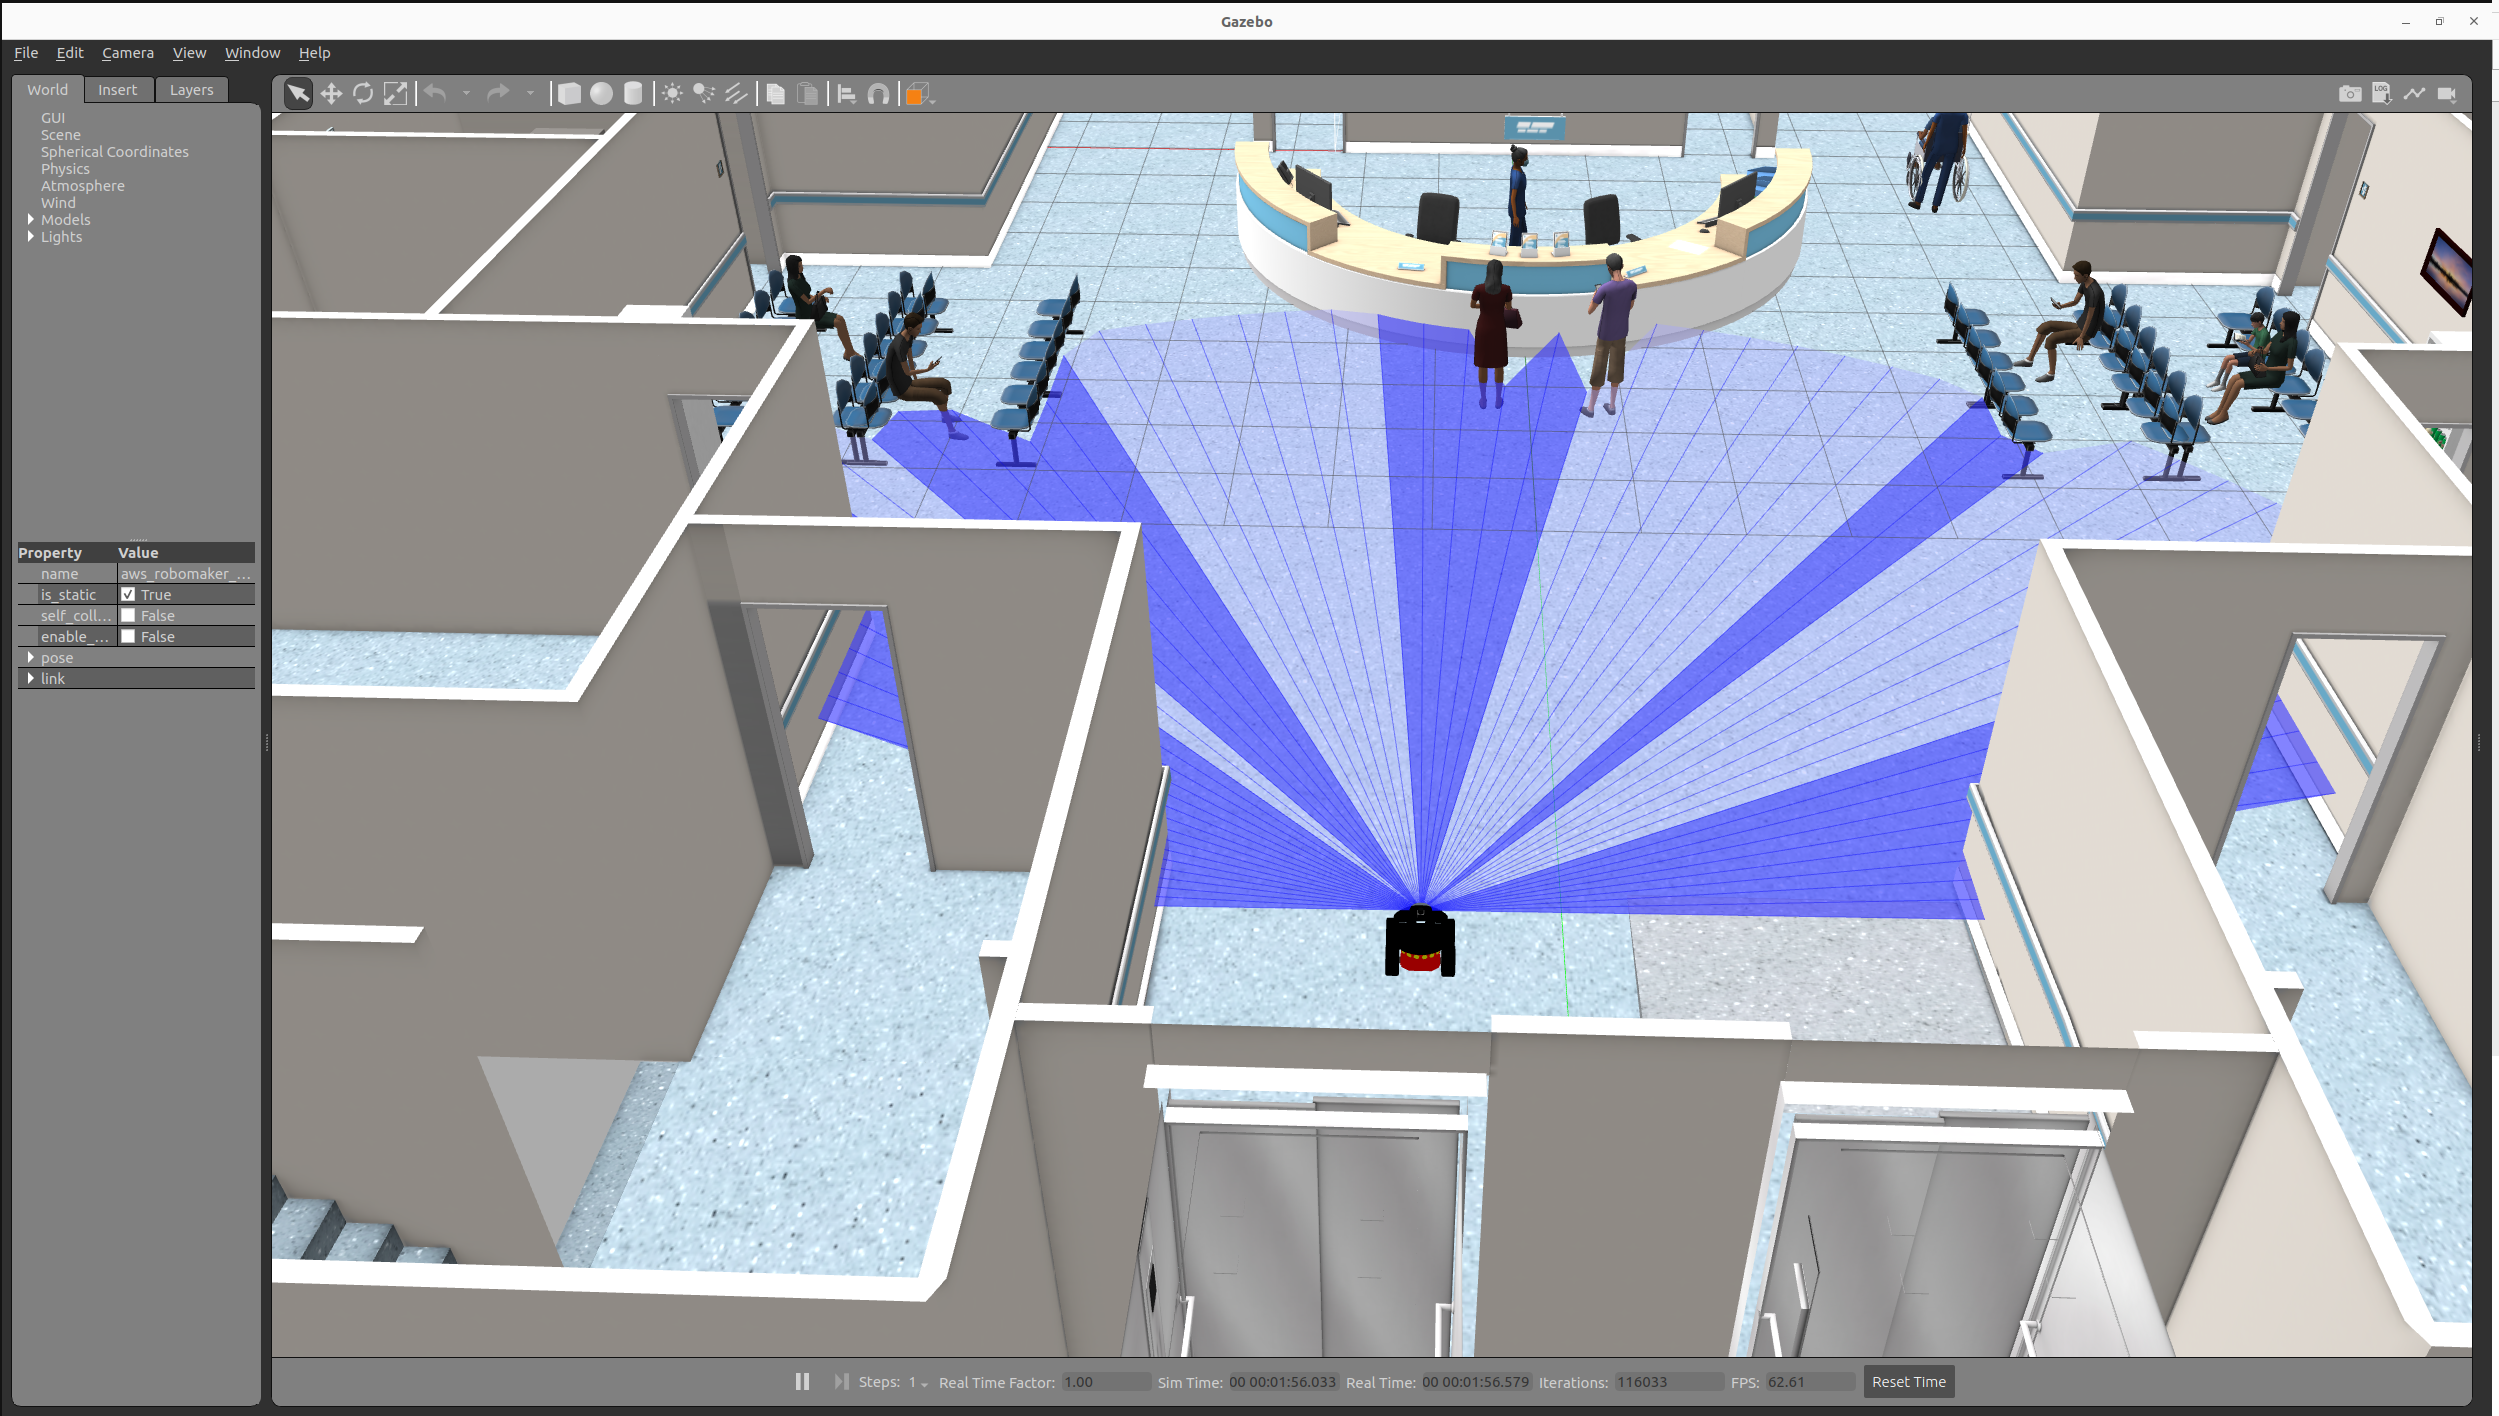
\includegraphics[width=0.8\columnwidth,keepaspectratio]{agent.png}
\caption{Environment with Pioneer 3AT, a 4-wheel differential drive agent}
\label{fig:your_label}
\end{figure}




\section{Literature Review}
Reinforcement learning (RL) has emerged as a promising approach for robot path planning and navigation in recent years. Compared to traditional path planning methods like A*, RRTs, etc., RL does not require an explicit map of the environment and can learn policies that generalize well to new environments.\par
    Q-learning is one of the most commonly used RL algorithms. Faust et al. (2018)\cite{faust2018prm} proposed a hierarchical planning method for long-range navigation tasks, that combines sampling- based path planning(PRM) with RL agents to complete tasks in very large environments. Which showed that PRM-RL expands the capabilities of both RL agents and sampling-based planners. The benefit here is that, although the RL agent depends on the robot and the goal, it is not dependent on the environment and can be used to create roadmaps for a variety of contexts.\par 

    
    Policy gradient methods like PPO can handle continuous action spaces and have also been applied for path planning. Tai et al. (2017)\cite{tai2017virtual} used PPO to train a policy for navigation in simple 2D environments with continuous control of velocity and steering angle. The policy was trained using only laser scan data as input.\par  

    
    Imitation learning from expert demonstrations can speed up training of navigation policies. Pfeiffer et al. (2017)\cite{pfeiffer2017perception} used behavior cloning with CNNs to imitate an A* planner and then fine-tuned the policy with RL. Demonstration was done that the learned navigation model is directly transferable to previously unseen virtual and, real-world environments. The method outperformed learning from scratch.\par 

    The question of whether policies developed in simulation using deep reinforcement learning could be used in the actual world was explored by Tzeng E. (2017)\cite{tzeng2017adapting}. As compared to policies trained using sparse real-world data, he shows in his research that vision systems trained on simulated data and adapted using our technique may be utilized to initiate deep visuomotor policies that achieve greater performance on real-world tasks.\par  

    
    Key challenges for RL navigation include sample efficiency, sim-to-real transfer, and integration with traditional methods for complementary capabilities. Hybrid methods that combine learning and classical planning are an active area of research.\par


% \begin{figure}[!htb]
% \centering
% \includegraphics[width=0.8\columnwidth,keepaspectratio]{grid.png}
% \caption{Multi-Agent Robots}
% \label{fig:your_label}
% \end{figure}



% \section{Proposed Solution}

% \subsection{Methodology}
% For the proposed project, we will conduct a comparative analysis between Proximal Policy Optimization (PPO) and Deep Q-Networks (DQN) for robotic motion planning in a static environment, utilizing LiDAR data for real-time navigation. The robotic platform will be equipped with LiDAR sensors, with the data processed into a state representation suitable for reinforcement learning. We will implement PPO and DQN algorithms, training both on identical tasks and environments to ensure comparability. The training will involve interaction with the environment to optimize action selection towards goal achievement while minimizing collisions. Key performance metrics such as success rates, episode length will be measured and analyzed to assess the effectiveness of each algorithm. The outcome will highlight the strengths and limitations of PPO and DQN in static environment navigation, guiding the choice of the optimal approach for practical robotic applications.




% \subsection{Environment Setup}






% In our project, we have chosen to utilize the "AWS robomaker-hospital-world" as the 3D environment in which our Reinforcement Learning (RL) agent will be deployed. This environment simulates a generic hospital floor, complete with a variety of objects and even simulated people. The primary robotic platform employed in this setup is a Pioneer 3AT Mobile Robot, equipped with a 4-wheel differential drive system. This configuration allows the robot to navigate and interact within the simulated hospital environment effectively. Further, original robot model will be slightly modified to add the 180° laser which will be utilized for obstacle detection in the environment.\\
% Additionally, Gazebo is employed to simulate the environment and the robot, which comes with
% a set of libraries that allow integration with ROS2 Humble framework.



\section{Methodology}

\subsection{Environment Setup}
In our study, we focus on training a reinforcement learning (RL) agent to navigate short distances within a simulated environment, specifically a hospital setting, without prior knowledge of the space's large-scale topology. This  integrates the RL agent into existing path planning algorithms as a local planner. The environment is a 3D representation of a hospital, complete with various objects and human figures, and is simulated using Gazebo, which integrates seamlessly with ROS2 Humble. Our chosen robotic platform is the Pioneer 3AT, a four-wheeled robot equipped with a 180° laser rangefinder providing 61 distance measurements ranging from 0.08 to 10 meters. This setup allows the robot to determine its position in space relative to a fixed Cartesian system and execute movement commands based on specified angular and linear velocities.

The RL agent's objective is to navigate to short-range goals (up to 10 meters) within this simulated environment, avoiding obstacles and fulfilling task constraints. The agent operates under specific conditions: it limits its angular speed to [-1,1] rad/s and linear speed to [0,1] m/s, with no backward motion. Collision detection is crucial and is determined when any laser measurement falls below 0.25 meters, considering the robot's geometry in relation to the laser's position. The target is defined as a point in the (x, y) space, and task completion is acknowledged when the robot comes within 0.40 meters of the target, a distance that accounts for the laser's position ahead of the robot's center and an additional safety margin.

\subsubsection{\textbf{OpenAI-Gym Setup}}
The RL agent is developed and trained using OpenAI Gym, an open-source toolkit that provides the necessary framework for creating a custom RL environment. The 3D models of the hospital and the Pioneer 3AT, slightly modified to include the 180° laser. This setup forms the foundation of our study, where the RL agent learns to navigate effectively in a static environment, representative of real-world conditions in a hospital setting.

%^{T_{FA}}
\textbf{Observation Space:} Defined as a dictionary, it includes:
\begin{itemize}
    \item Polar coordinates of the goal (\(r, \theta\)), with \(r \in [0, 60]\) meters and \(\theta \in [-\pi, \pi]\) radians.
    \item LIDAR sensor data, \(o_i\) for \(i = 1, \ldots, 61\), from the 180° LIDAR sensor with a depth of up to 10 meters.
\end{itemize}

\textbf{Action Space:} A 2-dimensional continuous array:
\begin{itemize}
    \item First element: Linear speed, within [0, 1] m/s.
    \item Second element: Angular speed, within [-1, 1] rad/s.
\end{itemize}

\textbf{Reward Function:} Implemented as a sparse reward strategy, the reward \( r_t \) at time \( t \) is defined as:
x`\begin{equation}
    r_t =
    \begin{cases} 
        1 & \text{if the goal is reached} \quad (r < 0.4), \\
        -1 & \text{if a collision occurs} \quad (\min_{i} o_i < 0.25), \\
        0 & \text{otherwise}.
    \end{cases}
\end{equation}
This design penalizes collisions and rewards goal attainment, fostering a risk-neutral policy.


\textbf{Step Method:} %Processes actions, updates the environment's state, captures new sensor data, and computes the reward based on the new state.
\begin{enumerate}
\item De-normalize the action to send the proper command to the robot
\item Send velocity command to the robot
\item Spin the node to allow sensor updates via callbacks
\item Transform coordinates to get polar coordinates of goal relative to robot
\item Get updated observation with laser readings and robot location
\item Get additional environment info
\item Compute reward
\item Check if episode is finished based on:
\begin{itemize}
\item Reaching goal (distance $<$ 0.4 m)
\item Collision detected (laser reading $<$ 0.25 m)
\end{itemize}
\item Return observation, reward, done flag, and info dict
\end{enumerate}

\textbf{Reset Method:} 

\begin{itemize}
\item Sample new start state:
\begin{itemize}
\item Randomly generate the initial state, including robot pose and target location, for the new episode based on a distribution. This introduces variety across episodes.

\end{itemize}

\item Reset simulation:
\begin{itemize}
\item Move the robot and update other entities in the simulation to the new start state. This is done by calling services and allowing time for the reset to fully propagate.
\end{itemize}

\item Initialize observation:

\begin{itemize}
\item Spin for sensor updates, transform coordinates, and construct the observation using the reset state. This creates the starting observation the agent sees.
\end{itemize}

\item Return observation:
\begin{itemize}
\item The observation is returned to the RL training algorithm so that the next episode can begin from the sampled start state.

\end{itemize}
\end{itemize}



\subsection{Learning Algorithms}

We implement two methods, Proximal Policy Optimization (PPO) and Actor Critic (A2C), to see which one works better for making a robot move in a fixed environment. We're using LiDAR data to help the robot navigate in real-time.

\textbf{Proximal Policy Optimization (PPO): }PPO has been designed to ensure that when updating the policy, the new policy doesn't deviate too far from the previous one. This is beneficial because drastic changes in the current policy parameters can lead to a significant drop in model performance, requiring many timesteps to recover the previous state. PPO is an on-policy algorithm applicable to both discrete and continuous action spaces. It comes in two variants: PPO-clip and PPO-penalty. We are concentrating on the first variant.

% \begin{equation}
%     \theta_{k+1} = \arg\max_{\theta} \mathbb{E}_{s, a \sim \pi_{\theta_k}} \left[ L(s, a, \theta_k, \theta) \right]
% \end{equation}

% \theta_{k+1} = \arg\max_{\theta} \mathbb{E}_{s, a \sim \pi_{\theta_k}} \left[ L(s, a, \theta_k, \theta) \right] \\

Note that the expectation is calculated over the state-action pair (a, s), where "a" represents the action sampled from the previous policy. A singular update is executed using Stochastic Gradient Descent (SGD), offering an alternative to traditional policy gradient descent. SGD significantly reduces computational effort by taking multiple smaller steps to adjust policy parameters. In each of these smaller steps, the gradient is computed using a mini-batch, a smaller sample, rather than considering all the sampled trajectories.

Let $r_t(\theta) = \dfrac{ \pi_{\theta}(a_t|s_t)} { \pi_{\theta_k}(a_t|s_t)}$. The the objective of PPO is the following equation:

\begin{strip}
  \begin{align}
    L^{CLIP}( \theta ) = \hat{ \mathbb{E}_{t} }     
                                            \Bigg[
                                                \min 
                                                (  
                                                  r_t(\theta)
                                                 \hat{A_t}
                                              ,
                                              \mathrm{
                                              clip(   
                                                    r_t(\theta)
                                               ,
                                               1 - \epsilon
                                               , 
                                               1 + \epsilon
                                                )
                                              }    
                                          \bigg)
                                           \hat{A_t}
                                            ) 
                                    \Bigg]
  \end{align}
\end{strip}

% \begin{strip}
%   \begin{align}
%       L(s, a, \theta_k, \theta) = \min 
%                                 \Bigg(
%                                      \dfrac{ \pi_{\theta}(a|s)} 
%                                      { \pi_{\theta_k}(a|s) }  
%                                       A^{\pi_{\theta_k}}(s, a)
%                                       ,
%                                       \mathrm{clip}
%                                       \bigg(
%                                            \frac{\pi_{\theta}(a|s)}{\pi_{\theta_k}(a|s)} 
%                                            ,
%                                            1 - \epsilon
%                                            , 
%                                            1 + \epsilon
%                                       \bigg)
%                                       A^{\pi_{\theta_k}}(s, a)
%                                 \Bigg)
%   \end{align}
% \end{strip}


\begin{enumerate}
    \item Positive Advantage ($A^{\pi_{\theta_k}}(s, a) > 0$): If the advantage of a state-action pair (a, s) is positive with respect to the old policy $\pi_{\theta_k}$, it is desirable to increase the probability of that action when in states. In doing so, the probability ratio $\dfrac{ \pi_{\theta}(a|s)} { \pi_{\theta_k}(a|s) }$ will be greater than one.\\

    The second part of the minimum function sets a limit on how much the probability ratio for a given state-action pair can increase. If this ratio exceeds $1 + \epsilon$, the clipped objective is chosen because it is lower than the unclipped one. This ensures that the growth in the likelihood of the action is constrained. Conversely, if the new parameters $\theta$ result in a policy that decreases the probability ratio even below $1 - \epsilon$, the unclipped term is selected. This decision is logical as it leads to a lower value of L, opposing the maximization goal of the algorithm. In such cases, the reduction in the probability ratio is not restricted.


    \begin{figure}[!htb]
    \centering
    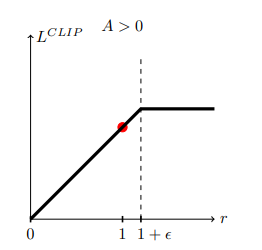
\includegraphics[width=0.6\columnwidth,keepaspectratio]{RL_project_update/positive.png}
    \caption{L-function with respect to the probability ratio when the
advantage A is positive}
    \label{fig:your_label}
    \end{figure}
    

    \item Negative Advantage ($A^{\pi_{\theta_k}}(s, a) < 0$): It is convenient to reduce the probability of the action a in state s when the relative advantage is negative.\\
    Similarly, in this scenario, the clipped objective constrains the reduction in the likelihood of the state-action pair. When the probability ratio of the new policy falls below $1 - \epsilon$, the second term of the minimum function is chosen, ensuring a controlled decrease in the action likelihood. Conversely, if the ratio is positive, the unclipped term is selected, allowing the penalization of such a policy to be unbounded. It's important to note that, given the negative nature of the advantage, increasing the likelihood of the action is undesirable.

    \begin{figure}[!htb]
    \centering
    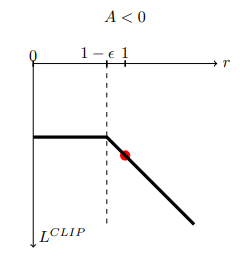
\includegraphics[width=0.6\columnwidth,keepaspectratio]{RL_project_update/negative.png}
    \caption{L-function with respect to the probability ratio when the
advantage A is negative}
    \label{fig:your_label}
    \end{figure}
    
\end{enumerate}


To ensure that the agent explores new states of the environment, an entropy bonus is incorporated into the loss function L. The influence of this component can be controlled by tuning the entropy coefficient. In essence, a higher coefficient increases the likelihood that the agent favors a random action rather than sampling from the current policy. As training progresses, the entropy bonus diminishes, ensuring that the agent's behavior gradually converges towards its existing policy over time.

Further, to update the policy, we need information about the on-policy value function. Since it involves an expectation, we can calculate it using a suitable estimator. In the case of PPO, an estimator with parameters is utilized, and these parameters ${\theta}$ are adjusted at each step of the algorithm. The pseudocode for the algorithm is provided below:


% \begin{figure}[!htb]
% \centering
% 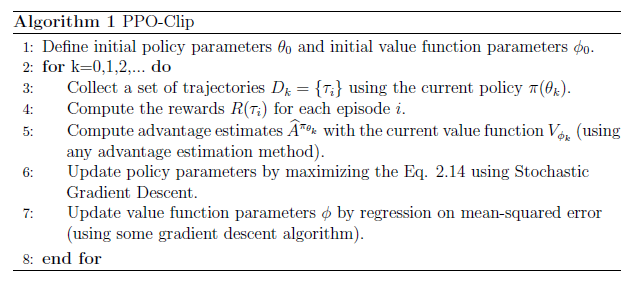
\includegraphics[width=0.8\columnwidth,keepaspectratio]{RL_project_update/PPOcode.png}
% \caption{Pseudocode of PPO-Clip}
% \label{fig:your_label}
% \end{figure}

\begin{figure}[!htb]
\centering

\includegraphics[width=\columnwidth, height=\columnwidth,keepaspectratio]{RL_project_update/a2c_only.png}
\label{fig:your_label}
\end{figure}


\begin{algorithm}
\caption{PPO-Clip}\label{ppo_psuedocode}

\begin{algorithmic}[1]

\State Define initial policy parameters $\theta_0$

\For{k=0,1,2,...}

\State Collect a set of trajectories $D_{k} = {\tau_{i}}$

\State Compute the rewards $R(\tau_{i})$ for each episode i

\State Compute advantage estimate $\hat{A}^{\pi_{\theta_{\kappa}}}$ with the current value function $V_{\phi_{\kappa}}$ (using any advantage estimation method)

\State Update policy parameter by maximizing using the Gradient Descent

\State Update the value function parameters $\phi$ by regression on mean-squared error (using some gradient descent algorithm)

\EndFor

\end{algorithmic}

\end{algorithm}

\textbf{Advantage Actor-Critic Network (A2C):}
\smallskip

We implement actor critic network as it has following advantages:

\begin{itemize}
    \item Sequential Decision Making: Mobile robots often operate in dynamic environments where they need to make a sequence of decisions over time to achieve a goal. A2C, being a sequential decision-making algorithm, is designed to handle such scenarios.

    \item Combining Value and Policy Learning: A2C combines the advantages of both value-based methods (e.g., Q-learning) and policy-based methods. It maintains both a value function (critic) and a policy (actor), allowing for a more stable and efficient learning process

    \item Efficient Exploration-Exploitation Trade-off: A2C includes a mechanism to balance exploration and exploitation. This is crucial for a mobile robot in an environment where it needs to explore to discover optimal paths but also exploit known information to achieve its goals efficiently.

    \item Adaptability: A2C is adaptable to different types of problems and can handle continuous action spaces, making it suitable for motion planning tasks where the robot's actions may be continuous.
\end{itemize}


\subsection{Training of the Agent}
The training process of the agent is illustrated below.
\subsubsection{Increasing simulation speed}
In general, RL is very sample inefficient. Many time steps are needed to get the ideal course of action. It therefore seems prudent to accelerate the simulation time as much as feasible. The training algorithm can handle more time steps in the same amount of time in this way. Two world file parameters can be changed in Gazebo to modify the simulation time:
\begin{itemize}
    \item Max step size (default value: 0.001 seconds), determining the  time in the simulation to be simulated in one step
    \item  Real time update rate (default value: 1000 Hz), which determines the minimum time period after which the next simulation step is triggered.
\end{itemize}
But you can't keep raising this parameter indefinitely. It's obvious that the algorithm's computational effort is limited by the amount of processing power the computer can handle. 
Our initial attempt at parameter adjustment resulted in a 15x quicker training pace for the first agent, with the maximum step size increased to 0.05 seconds and the real-time update rate to 3000 Hz. 
Moreover, the graphics output was disabled during training using a special Gazebo start file in order to lower the computational load on the system. \par
Ubuntu 22.04 LTS is installed on the machine that runs the training algorithm, a 12th Gen Intel® CoreTM i9-12900H × 20 with 16 GB of RAM. 


% \subsubsection{Tuning the hyperparameters}
% Proper tuning of the hyperparameters is crucial prior to training an RL agent, since default values may not be appropriate in all scenarios. To do so, the Python library Optuna is employed.
% Many of the parameters that can be changed with Stable Baselines 3, have been left mostly at their default values. Following parameters are selected to optimize using Optuna:
% \begin{itemize}
%     \item learning rate (default: 0.0003): the gradient update step size α ;
%     \item n steps (default: 2048): the number of steps to run per policy update;
%     \item gamma (default: 0.99): discount factor γ to compute the infinite-horizon discounted return;
%     \item clip range (default: 0.02): clipping parameter ε of the loss function;
%     \item gae lambda (default: 0.95): factor to regulate the bias-variance trade-off for Generalized Advantage Estimator;
%     \item ent coef (default: 0.0): used to compute the entropy bonus;
%     \item vf coef (default: 0.5): value function coeficient for the loss calculation.
% \end{itemize}


\subsubsection{Training on a simplified environment} 
To assess the efficacy of the chosen reward function, a simplified environment with no LIDAR samples was analyzed at the start of the training phase.
The goal of such a simplified setup is to debug undesirable behaviors in the Gym environment and ensure that the chosen reward function results in the desired policy. Later, more complexity can be added to the problem so that more sophisticated agents can be trained. The changes made for the simplified environment are listed below.\par
\begin{itemize}
    \item The observation space contains only the polar coordinates of the target (r, $\theta^{T}$, FA ) relative to the robot.
    \item  An episode ends if the robot reaches the target $(r > 0.4)$ or if it goes 3.5 meters farther than the target $(r > 3.5)$, creating a navigation limit.
    \par The reward function only returns 1 when the robot reaches the target, in all the other cases it returns 0.
\end{itemize}
The maximum number of steps is set to 1000 timesteps before beginning the training process. Given that the agent can travel up to 0.1 meters in a single step and that the agent is placed 3 meters away from the obstacle, the robot could complete the task in as few as 30 steps. As a result, 1000 steps per episode are more than enough to complete the task successfully.

It has been observed that the trained robot's behavior corresponds to intuition. In fact, the agent points directly to the target and arrives there without changing direction. All of this is evidence that the reward function selected can effectively lead to the desired policy. The following step is to train an agent by incorporating laser readings into the state.
\subsubsection{Training for the standard task}
The objective is to train an agent that can do the earlier described task, in which laser readings are additionally included in the state and a collision results in a negative reward. At this point, the procedure is broken down into multiple phases where the task's complexity gradually rises. By doing this, it is ensured that the training process is better understood and that any potential problems are easier to find.
\begin{itemize}

    % \item First-generation agent: \par
    % The robot is placed in an area that is almost entirely free of obstacles, the initial positions of the robot and the target are slightly modified at the start of each episode by adding a small random component to their coordinates. The agent is always placed 3-6 meters away from the goal.
    % The parameters chosen are as shown in the \ref{table:your_label}: 
    % % \begin{itemize}
    % %     \item  learning rate = 0.0001177 (default: 0.0003)
    % %     \item  n steps = 2279 (default: 2048)
    % %     \item gamma = 0.9880615 (default: 0.99)
    % %     \item clip range = 0.1482 (default: 0.02)
    % %     \item gae lambda = 0.9435888 (default: 0.95)
    % %     \item ent coef = 0.0000968 (default: 0.0)
    % %     \item vf coef = 0.6330533 (default: 0.5)
    % % \end{itemize}


    \begin{table}[]
    \centering
    \begin{tabular}{|l|l|l|}
    \hline
    \textbf{Step}            & \textbf{Error} &  default \\ \hline
     learning rate     &  0.0001177 &  0.0003        \\ \hline
    n steps             & 2279 &  2048         \\ \hline
    gamma               &  0.9880615 &  0.99        \\ \hline
    clip range          & 0.1482 & 0.02        \\ \hline
    gae lambda       & 0.9435888 &  0.95       \\ \hline
    ent coef       & 0.0000968 &  0.0         \\ \hline
    vf coef        & 0.6330533 &  0.5        \\ \hline
    \end{tabular}
    \caption{Hyper-parameters for first generation agent}
    \end{table}


% \begin{table}[!h]
%     \caption{Comparative Evaluation Metrics for Different Models}
%         \label{tab:my-table}
%         \begin{tabular}{|c|c|c|}
%         % \hline & \multicolumn{2}{|c|}{ \textbf{Standard} } & \multicolumn{2}{|c|}{ \textbf{Modified} } \\
%         \hline & F-beta & MAE & F-beta  \\
%         \hline {\textbf{U2Net}} & 0.865 & 0.045 & \textbf{--} & \textbf{--} \\
%         \hline {\textbf{U2Net\_Inside}} & 0.875 & 0.043 & 0.8348 & 0.051 \\
%         \hline {\textbf{U2Net\_Outside}} & 0.868 & 0.045 & 0.8196 & 0.053 \\
%         \hline {\textbf{U2net\_both}} & \textbf{0.887} & \textbf{0.039} & 0.8421 & 0.050 \\
%         \hline
%     \end{tabular}\\
% \end{table}


    The results and graphs mentioned in the report are from the first generation agent. 
    

    \item Second-generation agent: \par
    We are planning to train agent on a more heterogeneous set of episodes that recognizes different patterns of obstacles through its laser readings. Many different locations will be defined during the Gym environment's initialization by specifying the coordinates of the initial robot position and the target.

    \item Risk-seeker agent: \par
    We are planning to make the robot less sensitive to far away obstacles, a different reward function will be defined for the Risk-seeker agent.




\begin{figure}[!htb]
\centering
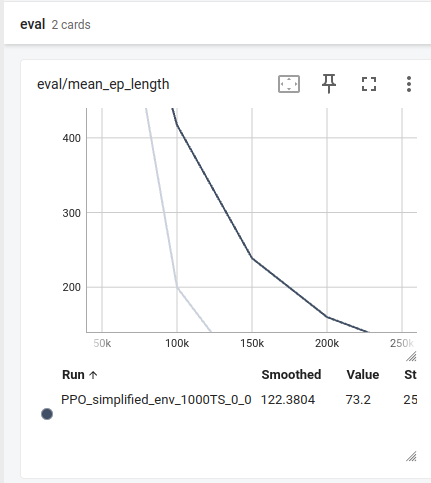
\includegraphics[width=0.8\columnwidth,keepaspectratio]{RL_project_update/simplified_env_episode_length.png}
\caption{Mean Episode Length for Simplified Environment}
\label{fig:your_label}
\end{figure}

\begin{figure}[!htb]
\centering
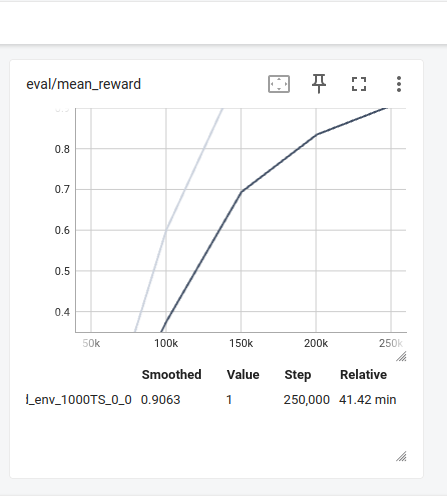
\includegraphics[width=0.8\columnwidth,keepaspectratio]{RL_project_update/simplified_env_reward.png}
\caption{Mean Reward for Simplified Environment}
\label{fig:your_label}
\end{figure}


\begin{figure}[!htb]
\centering
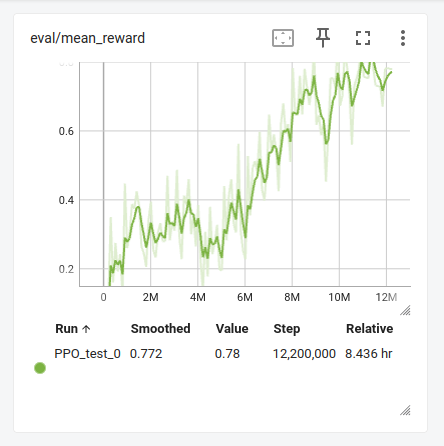
\includegraphics[width=0.8\columnwidth,keepaspectratio]{RL_project_update/mean_reward.png}
\caption{Mean Reward for Complex Environment  - PPO}
\label{fig:your_label}
\end{figure}


\begin{figure}[!htb]
\centering
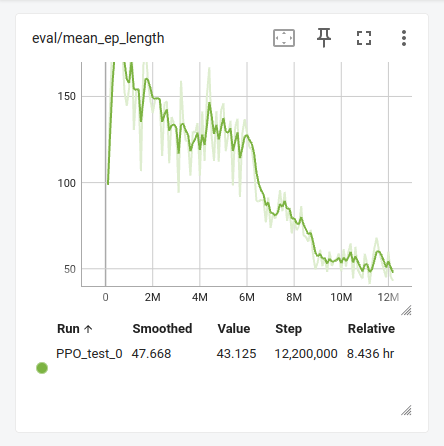
\includegraphics[width=0.8\columnwidth,keepaspectratio]{RL_project_update/man_ep_length.png}
\caption{Mean Episode Length for complex Environment - PPO}
\label{fig:your_label}
\end{figure}

\begin{figure}[!htb]
\centering
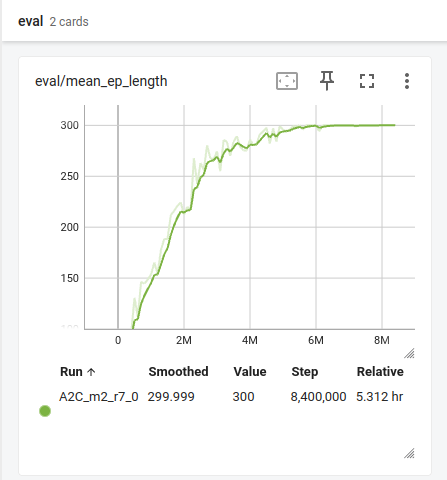
\includegraphics[width=0.8\columnwidth,keepaspectratio]{RL_project_update/A2C_results1.png}
\caption{Mean Episode Length for complex Environment - A2C}
\label{fig:your_label}
\end{figure}

\begin{figure}[!htb]
\centering
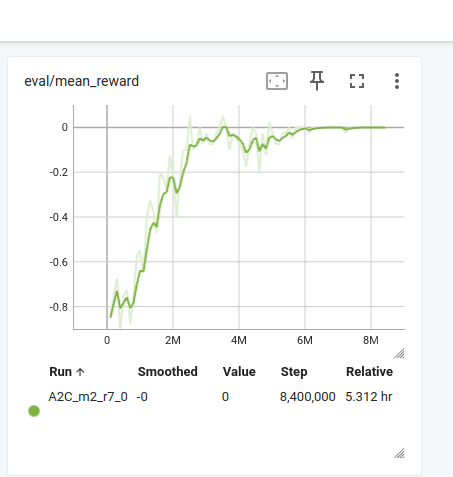
\includegraphics[width=0.8\columnwidth,keepaspectratio]{RL_project_update/A2C_results2.png}
\caption{Mean Episode Length for complex Environment - A2C}
\label{fig:your_label}
\end{figure}

\end{itemize}


\section{Applications}

\begin{enumerate}
    \item Mobile Robots in Healthcare: Robots used in healthcare settings for tasks like medication delivery and patient assistance can benefit from RL-based navigation to ensure safe and precise movement in clinical environments.

    \item Warehouse Automation: Autonomous robots in warehouses and fulfillment centers use RL to efficiently navigate and pick items from shelves, optimizing the logistics process.

    \item Autonomous Vehicles: Self-driving cars and autonomous drones use reinforcement learning for navigation. These vehicles learn to make decisions like lane changes, speed adjustments, and avoiding obstacles based on sensory data from cameras, LIDAR, and other sensors.

\end{enumerate}

\section{Result}
We discuss the short ranger path planning results here for PPO and A2C. 
In-case of PPO in training performance we got mean reward more than 0.8 as shown in the Fig. 7 for the simplified environment and the mean episode length converged to 73.2, which states that agent was successful in not only planning the path from spawn location to designated goal location but also finding the optimum path eventually.\par
For complex environment the PPO algorithm, initially for 5 million training steps gave unsatisfactory results of 0.4 rewards but after around 6 million training steps the agent showed good rise in the reward and after 12 million training steps final reward was of 0.78 and mean episode length converged to 43, which was better than the result from simplified environment. This demonstrates that with more number of training steps this algorithm can perform better with finding optimum path between start to goal. Which illustrates that PPO is suitable for short range path planning application.\par
On the other hand, A2C has not shown promising results in terms of planning path to goal location though the agent learned to prolong the episode length and navigate in the environment avoiding obstacles. Fig. 9 shows that the mean episode length value was 300 (the maximum episode length) after the 8.4 million training steps and the reward which was initially negative till 3 million steps converged to 0 reward. The potential reason can be the sparse reward of attaining goal. The inference is supported by simulation as well.





% \begin{figure}[!htb]
% \centering
% 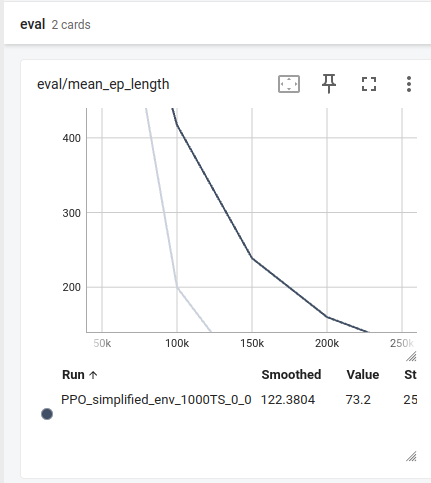
\includegraphics[width=0.8\columnwidth,keepaspectratio]{RL_project_update/simplified_env_episode_length.png}
% \caption{}
% \label{fig:your_label}
% \end{figure}





% \section{Goals}
% To develop and fine-tune a mobile robotic system that can plan and navigate autonomously in static environments using LiDAR data through the application of PPO and DQN algorithms.



% \section{Stretch Goals}

% The stretch goal of our project is to enable a mobile robot to navigate autonomously in dynamic environments and to implement the Advantage Actor-Critic (A2C) algorithm, comparing its effectiveness with PPO and DQN.

 \vspace{1cm}
 
% \section{Timeline and Division of Labour}

% \begin{table}[h]
% \centering
% \renewcommand{\arraystretch}{1.5}
% \caption{Timeline and Division of Labour}
% \label{table:your_label}
% \begin{tabularx}{\columnwidth}{|c|>{\hsize=1.5\hsize}X|>{\hsize=0.5\hsize}X|} 
% \hline
% \textbf{Timeline} & \textbf{Task} & \textbf{Task allocation} \\
% \hline
% Week 10 & Literature Review  \textbf{(Completed)} &  Prasanna, Shreya, Vaibhav, Shambhuraj \\
% \hline
% Week 11 & Literature Review\& Environment setup  \textbf{(Completed)}  & Shambhuraj, Prasanna, Shreya, Vaibhav\\
% \hline
% Week 12 & Implementing PPO  \textbf{(Completed)} & Shreya and Prasanna \\
% \hline
% Week 12 & Implementing DQN \textbf{(Completed)} & Vaibhav and Shambhuraj \\
% \hline
% Week 13 & Training PPO \& DQN \textbf{ (In Progress)} &  Prasanna, Shreya, Vaibhav, Shambhuraj \\
% \hline
% Week 14 \& 15 & Stretch goals and Documentation  \textbf{ (In Progress)} & Shreya Prasanna  Shambhuraj, Vaibhav\\
% \hline\end{tabularx}
% \end{table}
% \subsection{Division of labor}

% \cite{faust2018prm}

%%%%%%%%%%% Example 1%%%%%%%%%%%%%%%%%%%%%%%%%%
% \begin{thebibliography}{100} % 100 is a random guess of the total number of
% %references
% \bibitem{sharon2015conflictb} Faust, A., Ramirez, O., and Fiser, M., ``PRM-RL: Long-range Robotic Navigation Tasks by Combining Reinforcement Learning and Sampling-based Planning," \emph{ IEEE International Conference on Robotics and Automation (ICRA), 2018},  arXiv:1710.03937, Nov 2017.
% \bibitem{sharon2015conflictb} Tai, L., Paolo, G., and Liu, M., ``Virtual-to-real deep reinforcement learning: Continuous control of mobile robots for mapless navigation," \emph{ 2017 IEEE/RSJ International Conference on Intelligent Robots and Systems (IROS)}, Sep 2017.

% \bibitem{sharon2015conflictb} Pfeiffer, M., Schaeuble, M., and Nieto, J., ``From Perception to Decision: A Data-driven Approach to End-to-end Motion Planning for Autonomous Ground Robots," \emph{ 2017 IEEE International Conference on Robotics and Automation (ICRA)},   May 2017.

% \bibitem{sharon2015conflictb} Tzeng, E., Devin, C., and Hoffman, J., ``Adapting Deep Visuomotor Representations with Weak Pairwise Constraints," \emph{ under submission},  arXiv:1511.07111, May 2017.

% \bibitem{sharon2015conflictb} Garaffa, L., Basso, M., E., de Freitas, and Konzen, A., ``Reinforcement Learning for Mobile Robotics Exploration: A Survey," \emph{ IEEE Transactions on Neural Networks and Learning Systems},  10.1109/TNNLS.2021.3124466, Aug 2023.

% \end{thebibliography}

\section{Conclusion}
We designed two environments - a simplified and a complex one, with the later featuring more obstacles than the former. In our experiments, the Proximal Policy Optimization with Clip (PPO-Clip) algorithm demonstrated superior performance compared to the Advantage Actor-Critic (A2C) algorithm in both environments. 



\section{Future Scope}
Enhancing the agent's performance could be achieved through refining the reward function to be more specific or by incorporating a more diverse range of episodes in the training setting. However, owing to the constraints of the present study, additional research is necessary to pinpoint an optimal learning environment configuration.





\begin{thebibliography}{100} % 100 is a random guess of the total number of references
\bibitem{faust2018prm} Faust, A., Ramirez, O., and Fiser, M., ``PRM-RL: Long-range Robotic Navigation Tasks by Combining Reinforcement Learning and Sampling-based Planning," \emph{IEEE International Conference on Robotics and Automation (ICRA), 2018}, arXiv:1710.03937, Nov 2017.
\bibitem{tai2017virtual} Tai, L., Paolo, G., and Liu, M., ``Virtual-to-real deep reinforcement learning: Continuous control of mobile robots for mapless navigation," \emph{2017 IEEE/RSJ International Conference on Intelligent Robots and Systems (IROS)}, Sep 2017.
\bibitem{pfeiffer2017perception} Pfeiffer, M., Schaeuble, M., and Nieto, J., ``From Perception to Decision: A Data-driven Approach to End-to-end Motion Planning for Autonomous Ground Robots," \emph{2017 IEEE International Conference on Robotics and Automation (ICRA)}, May 2017.
\bibitem{tzeng2017adapting} Tzeng, E., Devin, C., and Hoffman, J., ``Adapting Deep Visuomotor Representations with Weak Pairwise Constraints," \emph{under submission}, arXiv:1511.07111, May 2017.
\bibitem{SchulmanWDRK17} Schulman J., Wolski F., Dhariwal P., Radford A., Klimov O., ``Proximal Policy Optimization Algorithms", https://arxiv.org/abs/1707.06347v2.
\bibitem{mnih2016asynchronous}
V.~Mnih, A.~Puigdom{\`{e}}nech Badia, M.~Mirza, A.~Graves, T.~P. Lillicrap, T.~Harley, D.~Silver, and K.~Kavukcuoglu, ``Asynchronous Methods for Deep Reinforcement Learning,'' \emph{CoRR}, vol. abs/1602.01783, 2016. [Online]. Available: http://arxiv.org/abs/1602.01783

\end{thebibliography}



% \bibitem{sharon2015conflictb}
% G. Sharon, R. Stern, A. Felner, en N. R. Sturtevant,
% ``Conflict-based search for optimal multi-agent pathfinding'',
% \textit{Artificial Intelligence}, vol 219, pp. 40–66, 2015.

% \section{Appendix}

% Contribution of team-members till current statge of project:
% \begin{enumerate}
%     \item \textbf{Literature Review:} Shambhuraj, Prasanna, Shreya
%     \item \textbf{2D Environment setup:} Shambhuraj, Prasanna
%     \item \textbf{Algorithm writing:} Shreya, Prasanna
%     \item \textbf{Documentation:} Shreya, Shambhuraj
% \end{enumerate}


\end{document}